
\documentclass[twoside,twocolumn]{article}

\usepackage{blindtext} % Package to generate dummy text throughout this template 

\usepackage[sc]{mathpazo} % Use the Palatino font
\usepackage[T1]{fontenc} % Use 8-bit encoding that has 256 glyphs
\linespread{1.05} % Line spacing - Palatino needs more space between lines
\usepackage{microtype} % Slightly tweak font spacing for aesthetics

\usepackage[english]{babel} % Language hyphenation and typographical rules

\usepackage[margin=0.5in,top=15mm,columnsep=10pt]{geometry} % Document margins
\usepackage[hang, small,labelfont=bf,up,textfont=it,up]{caption} % Custom captions under/above floats in tables or figures
\usepackage{booktabs} % Horizontal rules in tables

\usepackage{lettrine} % The lettrine is the first enlarged letter at the beginning of the text

\usepackage{enumitem} % Customized lists
\setlist[itemize]{noitemsep} % Make itemize lists more compact

\usepackage{abstract} % Allows abstract customization
\renewcommand{\abstractnamefont}{\normalfont\bfseries} % Set the "Abstract" text to bold
\renewcommand{\abstracttextfont}{\normalfont\small\itshape} % Set the abstract itself to small italic text

\usepackage{titlesec} % Allows customization of titles
\renewcommand\thesection{\Roman{section}} % Roman numerals for the sections
\renewcommand\thesubsection{\roman{subsection}} % roman numerals for subsections
\titleformat{\section}[block]{\large\scshape\centering}{\thesection.}{1em}{} % Change the look of the section titles
\titleformat{\subsection}[block]{\large}{\thesubsection.}{1em}{} % Change the look of the section titles

\usepackage{fancyhdr} % Headers and footers
\pagestyle{fancy} % All pages have headers and footers
\fancyhead{} % Blank out the default header
\fancyfoot{} % Blank out the default footer
\fancyhead[C]{ACSE - Group Project } % Custom header text
\fancyfoot[RO,LE]{\thepage} % Custom footer text

\usepackage{titling} % Customizing the title section

\usepackage{hyperref} % For hyperlinks in the PDF

\usepackage{graphicx} %package to manage images
\usepackage{subfigure}
\usepackage{caption}
\usepackage{subcaption}
\usepackage{booktabs}
\usepackage{float}

\usepackage[table,xcdraw]{xcolor}
\graphicspath{ {./images/} }
%----------------------------------------------------------------------------------------
%	TITLE SECTION
%----------------------------------------------------------------------------------------

\setlength{\droptitle}{-4\baselineskip} % Move the title up

\pretitle{\begin{center}\Huge\bfseries} % Article title formatting
\posttitle{\end{center}} % Article title closing formatting
\title{ANALYSIS REPORT FOR GORMANIUM RUSH} % Article title
}
}
\date{\today} % Leave empty to omit a date
\renewcommand{\maketitlehookd}{%
% \begin{abstract}
% \noindent \blindtext % Dummy abstract text - replace \blindtext with your abstract text
% \end{abstract}
}

%----------------------------------------------------------------------------------------

\begin{document}

% Print the title
\maketitle

%----------------------------------------------------------------------------------------
%	ARTICLE CONTENTS
%----------------------------------------------------------------------------------------
\lettrine[nindent=1em,lines=2]{T}he following report is based on the software designed to generate the best economic value during gormanium extraction . This software implementation generates optimum circuit configuration for given number of units. The mass balance calculator will tell the user the total concentration of gormanium and waste in the concentrate, and consequently the purity and recovery of the optimum solution based on the given input feeds of gormanium and waste. An economic analysis can be carried out to find the optimum values of recovery and waste depending on the given economic parameters. The code has four main parts:
\begin{itemize}
\item The Genetic Algorithm
\item The Mass Balance Solver
\item The Circuit Validity Checking, and finally
\item Post-Process and visualizations.
\end{itemize}

This report aims to highlight the optimization trends, the suitability and selection criteria of a set of generated circuit vectors to obtain maximum economic value based on fixed values of payment for recovery and penalty for impurities.



%------------------------------------------------
\section{RELIABILITY ANALYSIS}
On repeated testing we observe that when number of units(n) is greater than 5, we have a stable and robust algorithm that converges within the given iterations(200).
Following were the tests and their observations :
When the number of iterations were 8, for 100 consecutively generated vectors, we have 100 percent reliability for a range of max iterations from 200 to 1000 iterations. This means that our function converges to the global optimal within the given number of iterations for every run. \\
Similarly when number of iterations is 6, we see that our reliability is still strong at 100 percent for over 100 consecutive runs. \\
Now, we see that when we test for 5 iterations, we can observe some instability. Of the 100 iterations run, 70 converged. Thus we see a 70 percent reliability for five units.

\section{ANALYSIS OF SPEED OF CONVERGENCE}

The speed of convergence can be  affected by changing the probabilities of mutations and crossing in the code. We would expect faster convergence (fewer number of iterations) for higher probabilities. The trends observed meet this expectation. \\

\textbf{Mutation}

The figure below shows the impact of increasing the probabilities of mutation on the speed of convergence. When the difference in probabilities is large we can see a clear difference in trends.
\vspace{-4mm}
\begin{figure}[h]
\centering
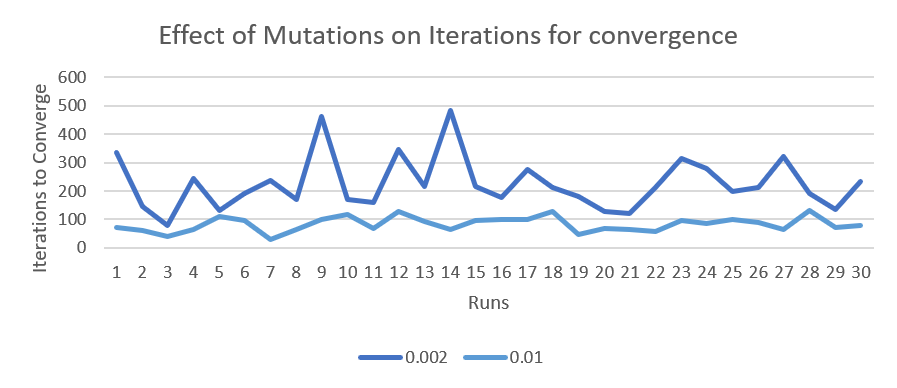
\includegraphics[height=4 cm\textwidth]{images/mutations comaprison.png}
\caption{Relatively High Probability of mutation leads to Lower Number of Iteration on Average}
\end{figure}

The figure below shows the area graphs for a range of probabilities. We can see that on average, the aforementioned trend still holds.
\vspace{-4mm}
\begin{figure}[h]
\centering
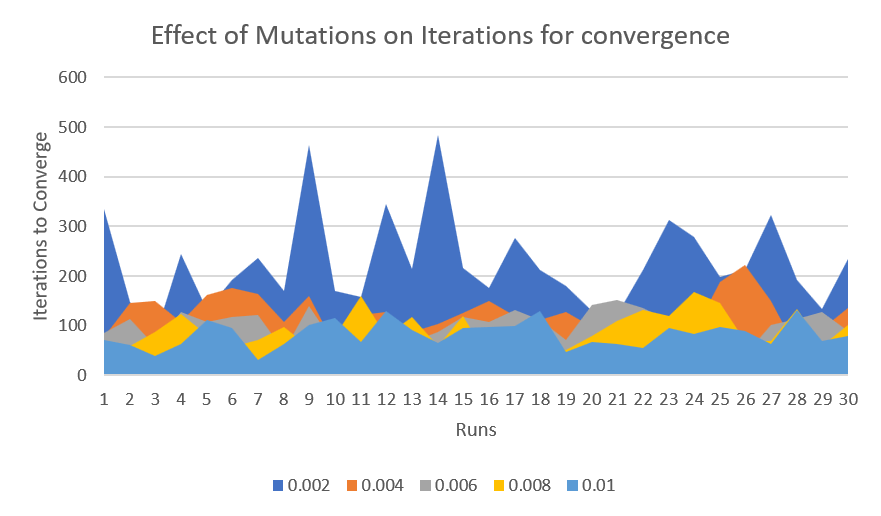
\includegraphics[height=6 cm\textwidth]{images/mutationsArea.png}
\caption{Area Graphs for Different Probabilities}
\end{figure}

This effect can also be quantified in terms of percentage decrease in the number of iterations and is represented by the graph below :

\vspace{-4mm}
\begin{figure}[h]
\centering
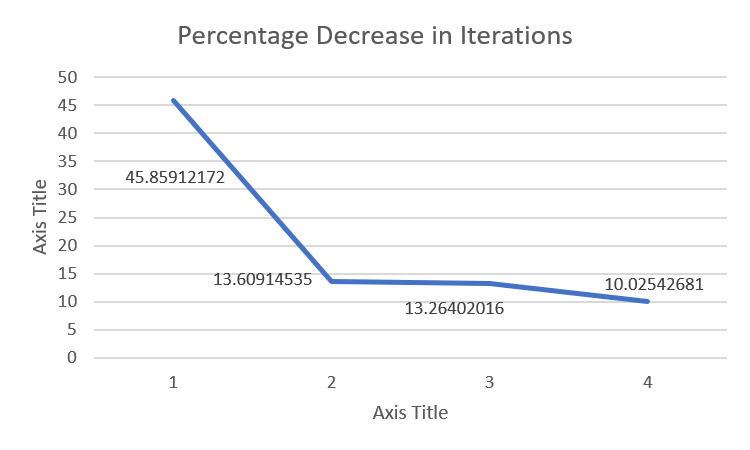
\includegraphics[height=6 cm\textwidth]{images/mutationsperdec.png}
\caption{Relatively High Probability of mutation leads to Lower Number of Iteration on Average}
\end{figure}

Thus we can observe that the effect of increasing mutation is significant on the speed of convergence.
The graph below shows 45\%, 13\%, 13\% and 10\%  decrease in number of iterations, on increasing the mutation by 0.2\% at each step.

\textbf{Crossings}


The figure below shows the impact of increasing the probabilities of crossings on the speed of convergence. Again, not unlike our observations for mutation variations, when the difference in probabilities is large we can see a difference in trends. However, unlike in the previous analysis the trends are less dramatic, which suggests that convergence is less sensitive to probability of crossing. 

\vspace{-4mm}
\begin{figure}[h]
\centering
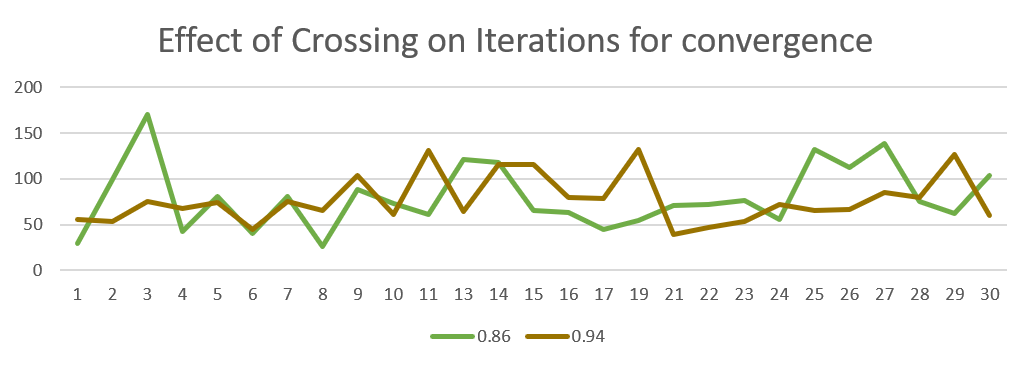
\includegraphics[height=3.5 cm\textwidth]{images/crossingComparisons.png}
\caption{Relatively High Probability of crossing leads to Lower Number of Iteration on Average}
\end{figure}

The figure below shows the area graphs for a range of probabilities. We can see that on average, the aforementioned trend still holds.
\vspace{-4mm}
\begin{figure}[h]
\centering
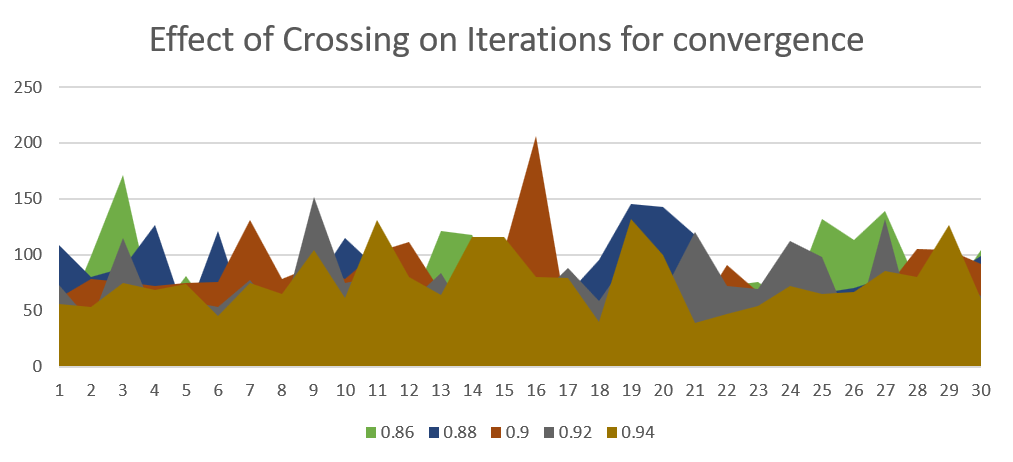
\includegraphics[height=4.5 cm\textwidth]{images/crossingarea.png}
\caption{Area Graphs for Different Probabilities of Crossing}
\end{figure}

%----------------------------------------------------------------------------------------

\section{Purity Vs Reliability}
As observed in the figure below, we can see that a fixed number of units(in our case n = 8), we observe a tradeoff between the purity of the concentrate and the amount of recovery that can be obtained.
\vspace{-4mm}
\begin{figure}[H]
\centering
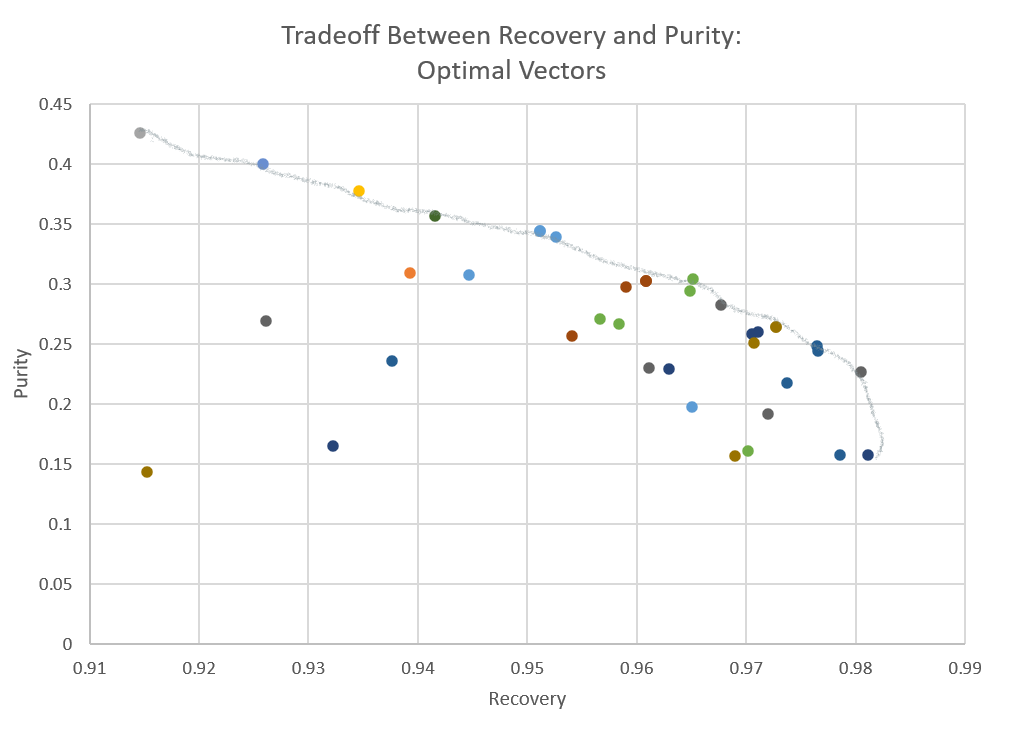
\includegraphics[height=6 cm\textwidth]{images/Picture1.png}
\caption{Boundary Setup and Edge Calculations Time}
\end{figure}
\vspace{-4mm}

The grey line shows the most optimal vectors with 8 units that can be selected for either given purity or a required amount of recovery.
Thus if we wish to obtain very high purity(higher on the y axis) we must sacrifice the amount of recovery and vice versa. Thus depending our economic parameters(payment for recovery and penalty for load) we can select the most suitable vector that leads to the most optimal combination.
Based on recorded Cw and Cw values and a fixed penalty of 100 and payment of 10 we can find the economic values for different feed inputs. \\
Here we can observe, for a fixed penalty and payment, we have the maximum economic value of 188.69 pounds/kg at Fg of 100 kg/s. \\
At this point the purity is 0.976507 and the recovery is 0.248469.  \\
However if we change our economic variables, we will observe that not only the feed, but also the level of purity and recovery will change. \\

%----------------------------------------------------------------------------------------
\section{Further Analysis}

\begin{itemize}
\item Further analysis must be carried out based on the trends observed in the optimal vectors generated. We must record all the vectors observed on the grey line in the figure above. We can then check to observe any similarities or trends in the type of vectors generated. This can also be used to further improve our validity functions.

\item For the economic analysis, we can further vary our parameters of payment and penalty to get different trends. We should be able to find the optimum input parameter(feed of gormanium) based on the observable maximum economic value obtained. This will also give us the obatined purity and recovery of the final concentrate


\end{itemize}



%----------------------------------------------------------------------------------------

\end{document}
